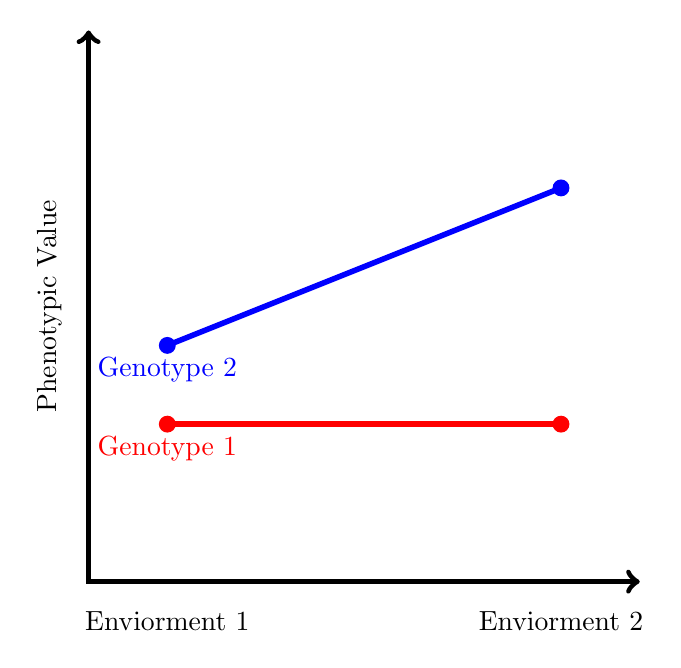
\begin{tikzpicture}
	% axes
	\draw[line width=2, black, <->] (7,0)  -- (0,0) --(0,7);

	% interaction
	\draw[line width=2, red] (1,2) node[below] {Genotype 1}-- (6,2);
	\draw[red, fill=red] (1,2) circle (0.1cm);
	\draw[red, fill=red] (6,2) circle (0.1cm);

	\draw[line width=2, blue] (1,3) node[below] {Genotype 2}-- (6,5);
	\draw[blue, fill=blue] (1,3) circle (0.1cm);
	\draw[blue, fill=blue] (6,5) circle (0.1cm);

	% text
	\node at (1,-0.5) {Enviorment 1};
	\node at (6,-0.5) {Enviorment 2};
	\node[rotate=90] at (-0.5,3.5) {Phenotypic Value};
\end{tikzpicture}
